%
% 	REWRITING OPEN GRAPHS
%	open graph rewriting
%	v1
%

% comment out when compiling 
%
%	REWRITING OPEN GRAPHS
%	preamble
%	v1

%  packages

\usepackage{amsfonts, amsthm, amssymb, amsmath, stmaryrd, etoolbox}
\usepackage{mathtools}
\usepackage{graphicx,caption,subcaption}
\usepackage{todonotes}
\usepackage{xcolor}
\usepackage{url}
\usepackage[inline]{enumitem}
	\setlist{itemsep=0em, topsep=0em, parsep=0em}
	\setlist[enumerate]{label=(\alph*)}
\usepackage[]{hyperref}
	\definecolor{hyperrefcolor}{rgb}{0,0,0.7}
	\hypersetup{colorlinks,linkcolor={hyperrefcolor},citecolor={hyperrefcolor},urlcolor={hyperrefcolor}}
\usepackage{tikz}
	\usetikzlibrary{matrix,arrows,shapes,decorations.markings,decorations.pathreplacing}
\usepackage[numbers]{natbib}
\usepackage{doi}

%
% commands
%

\newcommand{\RR}{\mathbb{R}}
\newcommand{\ZZ}{\mathbb{Z}}
\newcommand{\NN}{\mathbb{N}}
\newcommand{\QQ}{\mathbb{Q}}
\newcommand{\CC}{\mathbb{C}}
\newcommand{\DD}{\mathbb{D}}
\newcommand{\MM}{\mathbb{M}}
\renewcommand{\epsilon}{\varepsilon}

\newcommand{\defn}[1]{\textbf{#1}}
\newcommand{\op}[1]{\operatorname{#1}}
\newcommand{\cat}[1]{\mathbf{#1}}
\newcommand{\dblcat}[1]{\mathbb{#1}}
\renewcommand{\t}[1]{\text{#1}}

\newcommand{\from}{\colon}
\newcommand{\xto}[1]{\xrightarrow{#1}}
\newcommand{\sm}{\smallsetminus}
\newcommand{\tospan}{\xrightarrow{\mathit{sp}}}
\newcommand{\tocospan}{\xrightarrow{\mathit{csp}}}
\newcommand{\diagram}[1]{\raisebox{-0.5\height}{\includegraphics{#1}}}

\newcommand{\bispmap}[1]{\mathbf{Sp(#1)}}
\newcommand{\dblspmap}[1]{\mathbb{S}\mathbf{p(#1)}}
\newcommand{\bicspmap}[1]{\mathbf{Csp(#1)}}
\newcommand{\dblcspmap}[1]{\mathbb{C}\mathbf{sp(#1)}}
\newcommand{\bispsp}[1]{\mathbf{Sp(Sp(#1))}}
\newcommand{\dblspsp}[1]{\mathbb{S}\mathbf{p(Sp(#1))}}
\newcommand{\bicspcsp}[1]{\mathbf{Csp(Csp(#1))}}
\newcommand{\dblcspcsp}[1]{\mathbb{C}\mathbf{sp(Csp(#1))}}
\newcommand{\bimonspcsp}[1]{\mathbf{MonicSp(Csp(#1))}}
\newcommand{\dblmonspcsp}[1]{\mathbb{M}\mathbf{onicSp(Csp(#1))}}
\newcommand{\biepiccspsp}[1]{\mathbf{EpicCsp(Sp(#1))}}
\newcommand{\dblepiccspsp}[1]{\mathbb{E}\mathbf{picCsp(Sp(#1))}}
\newcommand{\spcsp}[1]{\mathbf{Sp(Csp(#1))}}
\newcommand{\dblspcsp}[1]{\mathbb{S}\mathbf{p(Csp(#1))}}

\newcommand{\LspanD}{ L \t{-} \operatorname{Span} ( \mathbf{D} ) }
\newcommand{\LopenD}{ L \t{-} \operatorname{Open} }
\newcommand{\LrewriteD}{ L \t{-} \operatorname{Rewrite} }

%
% math operators
%

\DeclareMathOperator{\Hom}{Hom}
\DeclareMathOperator{\id}{id}
\DeclareMathOperator{\ob}{Ob}
\DeclareMathOperator{\arr}{arr}
\DeclareMathOperator{\im}{im}
\DeclareMathOperator{\Aut}{Aut}
\DeclareMathOperator{\Bij}{Bij}
\DeclareMathOperator{\Sub}{Sub}
\DeclareMathOperator{\colim}{colim}

%
% envirnments and counters
%

\newtheorem{thm}{Theorem}[section]
\newtheorem{lem}[thm]{Lemma}
\newtheorem{prop}[thm]{Proposition}
\newtheorem{cor}[thm]{Corollary}

\theoremstyle{remark}
	\newtheorem{remark}[thm]{Remark}
	\newtheorem{notation}[thm]{Notation}

\theoremstyle{definition}
	\newtheorem{ex}[thm]{Example} 
	\newtheorem{df}[thm]{Definition}

% \setcounter{tocdepth}{1} % Sets depth for table of contents. 

%
% tikz types
%

\tikzset{->-/.style={decoration={%
			markings,
			mark=at position .5 with {\arrow{>}}},postaction={decorate}}
}
\tikzset{->-pos/.style={decoration={%
			markings,
			mark=at position #1 with {\arrow{>}}},postaction={decorate}}
}
\tikzset{->-/.style={decoration={%
			markings,
			mark=at position .5 with {\arrow{>}}},postaction={decorate}}
}
\tikzset{->-pos/.style={decoration={%
			markings,
			mark=at position #1 with {\arrow{>}}},postaction={decorate}}
}
 % input preamble
\bibliography{3--RewriteOpenGraphs--Bibliography}	

\section{Rewriting open graphs} % section title

% INTRODUCTION TO THE SECTION

In this section, we develop the theory
of double pushout rewriting on open graphs.
We closely follow the theory of
classical double pushout (DPO) rewriting 
on graphs as introduced by 
\todo{citatation}.
Because many good introductions
to the theory of DPO rewriting
already exist
\todo{citations},
we do not recall any of this
theory here.  
However, we do follow a
common trajectory in the 
organization of this paper.

First, we introduce the idea
of a rewrite rule, 
which in the DPO context goes 
by the name of a \emph{production}.
Roughly, a production states that
an open graph $G$ can be replaced
with another open graph $H$.
However, rewriting is really
about replacing sub-terms,
or, in our case, open subgraphs
with a new open subgraph.  
Thus, given a production that
rewrites $G$ to $H$,
we seek a condition that allows us to
remove any instance of $G$ as a
open subgraph and glue $H$
in its place.
For the categorically minded,
pushouts are the operation
one goes to when wanting to
`glue' things together. 
Indeed, this is where 
double pushouts enter the picture,
and our sough after condition
is the existence of 
a \emph{pushout complement}.
Combining a given production with
pushout complements allows us
to derive additional productions
in which we remove an
open subgraph and glue in
some new open subgraph,
all according to the initial production.

{\color{red} THIS IS MORE OF AN INTRO
TO THE PAPER BIT. COME BACK LATER TO EDIT}

A span of cospans is simply a 
commuting diagram of shape
\[
	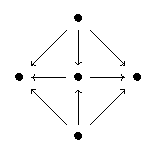
\includegraphics{InclGrphx--Diagram--SpanCospan}.
\]
In particular, a \emph{span of open graphs} 
is a commuting diagram of the form
%
\begin{equation}
\label{dgrm--SpanOpenGraphs}
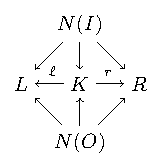
\includegraphics{InclGrphx--Diagram--SpanOpenGraphs}
\end{equation}
%
in the category $\cat{Graph}$.
Here, $N$ is the functor from \eqref{eq--FunctorN}
and $\ell$ and $r$ are 
the \defn{legs} of the span.

\begin{df}
	A \defn{rewrite rule} or \defn{production} 	
	is a span of open graphs with monic legs.
\end{df}

Within DPO graph rewriting
productions are defined using 
spans of graphs
with the theory developed considering
using spans with two monic legs,
only the left leg monic, and
arbitrary legs.
\todo{cite different authors for each case}
\todo{cite the paper comparing approaches}
When needing to distinguish 
between these different 
respective cases,
one ofter uses the terms
`linear production',
`left linear production', and  
`production'.
Because we have no need to 
consider different cases,
we take `production' to mean
a span of open graphs with 
two monic legs.

The conceit of a production,
take \eqref{dgrm--SpanOpenGraphs}
for instance,
is that we can replace the 
open graph 
\[
	N(I) \to L \gets N(O)
\]
with the open graph
\[
	N(I) \to R \gets N(O).
\]
This is desirable in many situations.
One particular setting would be
when using a graph to model
a network, for instance
a circuit of resistors.
There are many configurations
which have equal resistances, 
and so a budget conscious 
engineer would want to replace
a network with another
of equal resistance but
containing fewer resistors.
The application presented in 
Section \todo{put in the section number}
will involve string diagrams
for a Frobenius object.
Here, we will want to replace 
a given string diagram
(which is just an arrow in some category)
with any other as long as 
they are equal.

The benefit of conceptualizing
a production \eqref{dgrm--SpanOpenGraphs} 
as a span is that
it can serve as a mechanism
to identify instances of $L$
\todo{say we deonte open graph by G sometimes}
as an open subgraph, of say $G$,
and glue $R$ in its place.  
The role that $K$, 
which is a subgraph of both $L$ and $R$,
plays in this process is that its
elements remain fixed through the rewriting. 
In reality, when we are replacing $L$
with $R$ inside of $G$, 
all pieces of $L$ coming from $K$
are preserved.  
The fact the inputs $N(I)$ and 
outputs $N(O)$ factor through $K$
in a production ensures that
the interface is always preserved
under rewriting.  
While edges incident to the 
interface may be affected,
the nodes themselves remain untouched.  

This removing and replacing is made precise
using double pushouts.
First, however, we introduce a condition that 
ensures this operation can actually be done.

\begin{df}
	Given a production $p$
	\[
	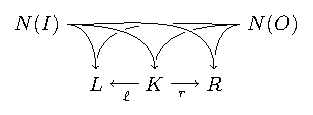
\includegraphics{InclGrphx--Diagram--Production2}
	\]
	a \defn{match} of $p$ inside 
	an open graph $G$ is a 
	morphism of open graphs 
	\[
		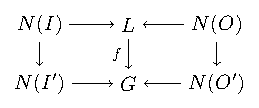
\includegraphics{InclGrphx--Diagram--Match}
	\]
	This match is said to
	satisfy \defn{the gluing condition}
	if there exists an open graph $D$ and
	open graph morphisms 
	$f' \from K \to D$ and $\ell' \from D \to G$
	such that the marked square in
	the commuting diagram
	\begin{equation}
	\label{dgrm--GlueCond}
		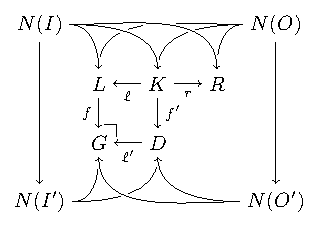
\includegraphics{InclGrphx--Diagram--GlueCond}
	\end{equation}
	is a pushout.
\end{df}

This differs from the usual
gluing condition only mildly. 
\todo{cite something here}
The only addition is that 
interfaces are respected,
hence the arrows from 
$N(I)$, $N(O)$, $N(I')$ and $N(O')$
in the above diagram. 

Whenever the gluing condition
is satisfied, we can replace
the instance of $L$ inside $G$
with $R$ resulting
in a new graph $H$.
To be precise, $H$ is a pushout, 
as situated in the diagram
\[
	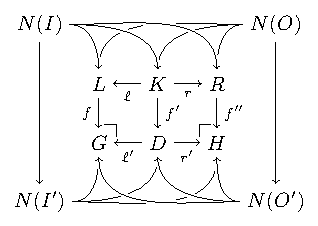
\includegraphics{InclGrphx--Diagram--DPO}
\]
Because this pushout is happening
in a topos, $\cat{oGraph}$,
both $\ell'$ and $r'$ are monic.
Hence
\[
	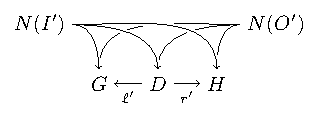
\includegraphics{InclGrphx--Diagram--DerivedProduction}
\]
is a production
which we say is \defn{derived} from $p$ and $f$.

\begin{df}
	An \defn{open graph grammar}, 
	or just \defn{grammar}, 
	is a pair $( \mathcal{ G } , \mathcal{ P } )$
	where $ \mathcal{ G } $ is a set of open graphs
	and $ \mathcal{ P } $ is a set of productions. 
	Given an open graph grammar,
	the collection of all productions 
	derived from any $ p \in \mathcal{ P } $ 
	and matching of 
\end{df}















